\section{Software}

\begin{frame}{Software}
	\begin{block}{Google Cast}
		Google Chromecast es un dispositivo que actúa como receptor y es compatible con el protocolo propietario Google Cast.
		Para iniciar la reproducción de un contenido pulsamos el botón de \textit{cast}.
	\end{block}

	\begin{figure}[h]
		\centering
		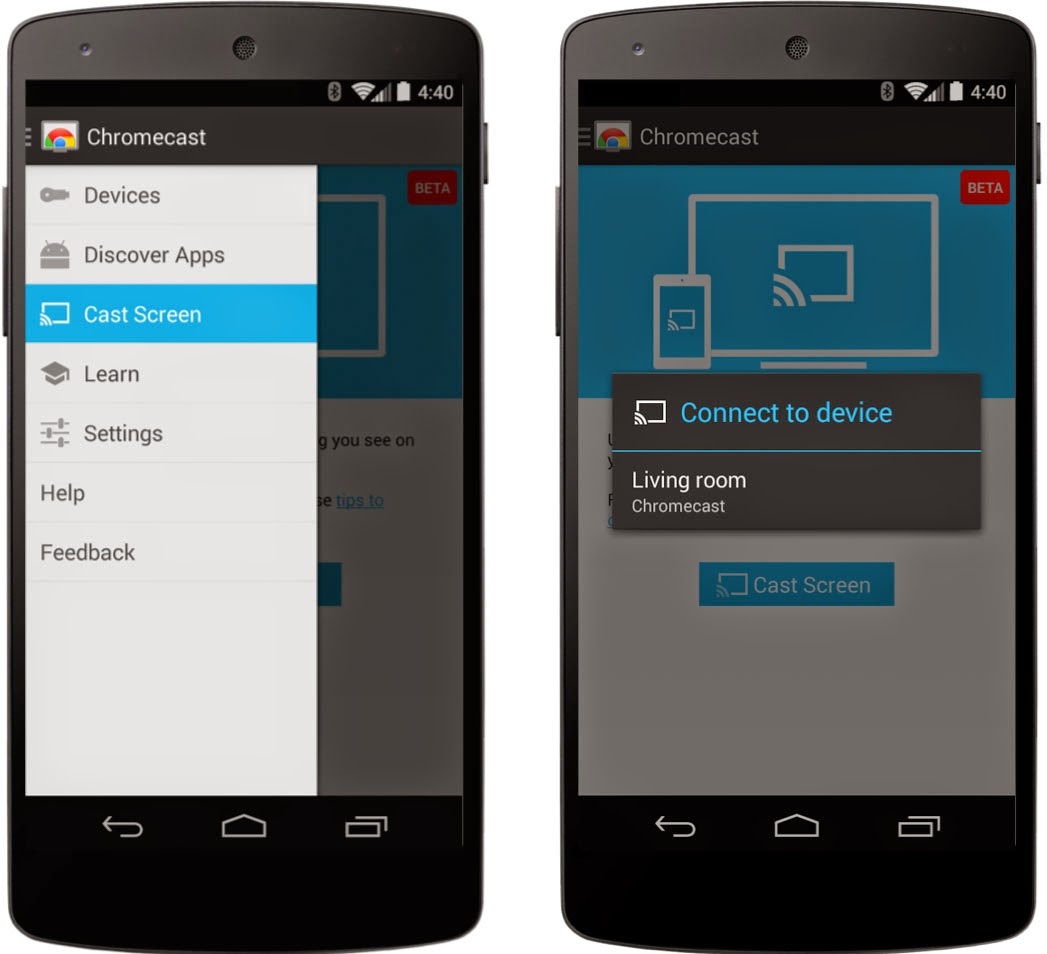
\includegraphics[width=0.5\textwidth]{./Imagenes/chromecast-mirroring.jpg}
	\end{figure}
\end{frame}



\subsection{Modos de funcionamiento}

\begin{frame}{Funcionamiento}
	\begin{block}{Primer modo}
		Usar el dispositivo emisor para controlar la reproducción. El receptor (ej: Chromecast) se encarga de descargarlo del servidor, liberando al emisor de esta tarea. 
		Esto permite al emisor ahorrar batería, estar bloqueado o en otra aplicación mientras la reproducción tiene lugar.
	\end{block}

	\begin{figure}[h]
		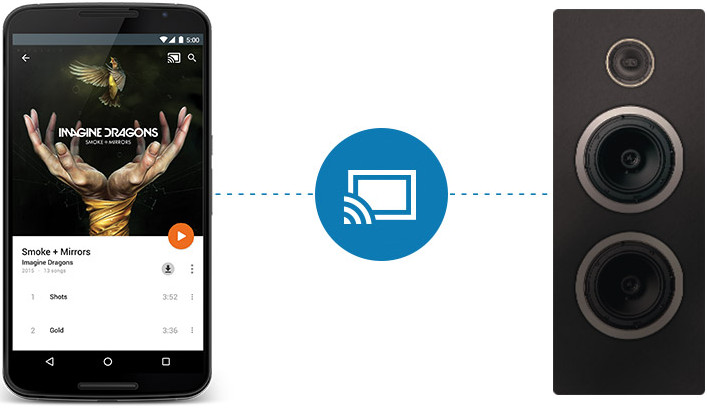
\includegraphics[width=0.65\textwidth]{./Imagenes/cast-speaker.jpg}
	\end{figure}
\end{frame}	
	
	
\begin{frame}
	\begin{block}{Segundo modo}
		Diseñado para enviar contenido del emisor, como cuando hacemos mirroring o usamos la televisión como segunda pantalla.
		
		La calidad del streaming en este caso varía según la potencia de procesamiento del emisor. En el caso de un smartphone la calidad
		de las imágenes normalmente se deteriora debido al escalado.
	\end{block}
	
	\begin{figure}[h]
			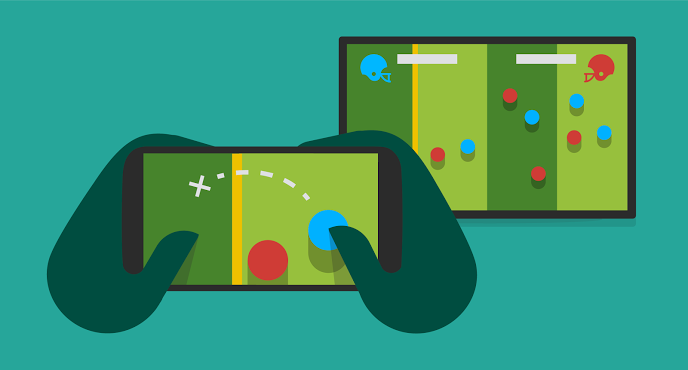
\includegraphics[scale=0.3]{./Imagenes/seconddisplay.png}
			\caption{Pantalla externa}\label{fig:seconddisplay}
	\end{figure}		
\end{frame}


\begin{frame}{Comparativa}
	\begin{minipage}[b]{.45\textwidth}
		\centering
		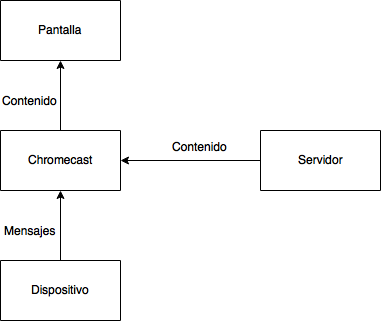
\includegraphics[scale=0.52]{./Imagenes/ChromecastModo1.png}
		%\caption{Primer modo}
	\end{minipage}\qquad
	\hspace{1.65cm}
	\begin{minipage}[b]{.3\textwidth}
		\centering
		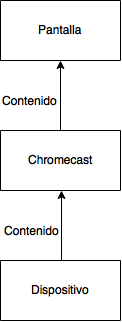
\includegraphics[scale=0.52]{./Imagenes/ChromecastModo2.png}
		%\caption{Segundo modo}
	\end{minipage}
\end{frame}



\subsection{Arquitectura}
\begin{frame}{Arquitectura}
	Google Cast implementa el paradigma del productor-consumidor.
	\begin{block}{ }
		La aplicación emisora se encarga de controlar la reproducción y elegir el dispositivo donde se emite el contenido. 
	\end{block}
	
	\begin{block}{ }
		La aplicación receptora es una aplicación web ejecutándose en una adaptación de Chrome.
		
		El código de la misma debe estar alojado en un servidor, ya que el Chromecast no almacena aplicaciones. Por tanto, aunque el contenido esté alojado en un dispositivo de la red local, seguirá necesitando conexión a internet para cargar la web app. 
	\end{block}
\end{frame}



